\chapter{Analyse et spécification des besoins}

La phase d’analyse et spécification des besoins présente une étape primordiale dans le cycle de développement d’un projet. En effet, elle permet de mieux comprendre le travail demandé en dégageant les besoins des différents utilisateurs que doit le système accomplir. Pour ce faire, dans le présent chapitre nous allons commencer par l’analyse des besoins en détaillant les besoins fonctionnels et non fonctionnels ensuite nous allons présenter les différents cas d’utilisation de l’application et en enfin nous exposons quelques diagrammes de séquence.

\section{Spécification des besoins}

Tout au long de cette section nous allons identifier les différents acteurs qui interagissent avec le système et nous allons énumérer les besoins fonctionnels ainsi que les besoins non fonctionnels.


\subsection{Les besoins fonctionnels}

Notre application doit offrir aux utilisateurs différentes fonctionnalités selon les privilèges de chacun d’entre eux. Ces besoins peuvent être résumés dans les points suivants: \\
\begin{itemize}
\item \textbf{BF1:} Le système doit permettre la gestion des rôles des différents intervenants dans l’opération d’apurement de la base de données. \\
\item \textbf{BF2:} Le système doit accéder aux champs NOTAM expirés de la base de données pour les faire supprimer.\\
\item \textbf{BF3:} Le système doit assurer que chaque opération effectuée doit être validée par un être supérieur, la validation finale doit être suivie par l’exécution de l’opération.\\
\item \textbf{BF4:} Le système doit assurer que chaque opération effectuée doit être enregistré dans un historique qui garde la nature de l’opération, celui qui l’a lancé et ceux qui l’ont validé.\\
\item \textbf{BF5:} Le système doit permettre à un super-administrateur de gérer la liste des différents utilisateurs ; ajouter un compte utilisateur en précisant son type, modifier un profile utilisateur ou bien le supprimer.\\
\end{itemize}

\subsection{Les besoins non fonctionnels}

En plus des besoins, plusieurs considérations et contraintes additionnelles doivent être prises en compte lors de la mise en place de l’application. Ces besoins peuvent se résumer par ce qui suit.

\subparagraph{Ergonomie et convivialité :} L'application doit présenter une interface claire conviviale et ergonomique.
\subparagraph{Maintenabilité :}Le système devra pouvoir être maintenu par des développeurs qui ne sont pas les développeurs d’origine.
\subparagraph{Vitesse de temps de réponse :}La réponse devra être assez rapide pour éviter d’interrompre le flux de pensée de l’utilisateur.
\subparagraph{Évolutivité :}La modularité et l'extensibilité de l'architecture de l'application en cas d'ajout des nouveaux services
\section{Analyse des besoins}

Pour spécifier de façon formelle les besoins requis par l’application, nous avons opté pour la réalisation du diagramme des cas d’utilisation pour avoir une meilleure compréhension des besoins.

\subsection{Identifaction des acteurs}

Dans cette partie, nous identifions les différents acteurs qui agissent sur notre application. En effet, un acteur est un élément externe, qui peut être un être humain, une machine, ou un autre système, qui interagit avec le système pour avoir un résultat.\\

Après avoir étudié les différentes interactions internes et externes du système nous avons jugé nécessaires les acteurs suivants :\\
\begin{itemize}
\item \textbf{Super-Administrateur:} le super-administrateur est un acteur qualifié d’une autorité principale d’accès. Il joue un rôle capital dans l’assurassions du bon fonctionnement du système. C’est la personne qui prend en charge la gestion des comptes des
utilisateurs ainsi la validation des opérations effectuées sur la base de données.\\
\item \textbf{Administrateur:} l'administrateur est un acteur qualifié d'une autorité moins importante que celle d super-administrateur. Cet acteur est chargé de faire les actions préliminaires de validation. Il suggère au super-administrateur l'ajout des comptes utilisateurs. Pour chaque site, on trouve une personne qui joue le rôle d'un administrateur. \\ 
\item \textbf{Agent: } un agent est un acteur principal en interaction directe avec l’application. Il s'agit de la personne qui manipule la base de données en direct. Il génére les messages. Il y a deux type d'agent: Un agent site centrale situé au niveau l AITC et un agent site distant situé au niveau des site aérien autre que l'AITC.\\

\end{itemize}

\subsection{Diagrammes cas d'utilisation}
Après avoir identifier les différents acteurs de notre système, nous réservons cette section pour illustrer le diagramme de cas d'utilisation pour chaque type d'acteur. \\

\subsubsection{Diagramme cas d'utilisation pour le super administrateur}
La figure ci-dessous illustre le diagramme cas d'utilisation pour un super administrateur. En effet, un super administrateur peut, après avoir s'authentifié, valider les opération requise par un agent, gérer les comptes des exploitant, forcer les opérations d'exception en cas d'urgent, et également communiquer avec les autres exploitants par des messages.
\begin{figure}[!h]
\begin{center}
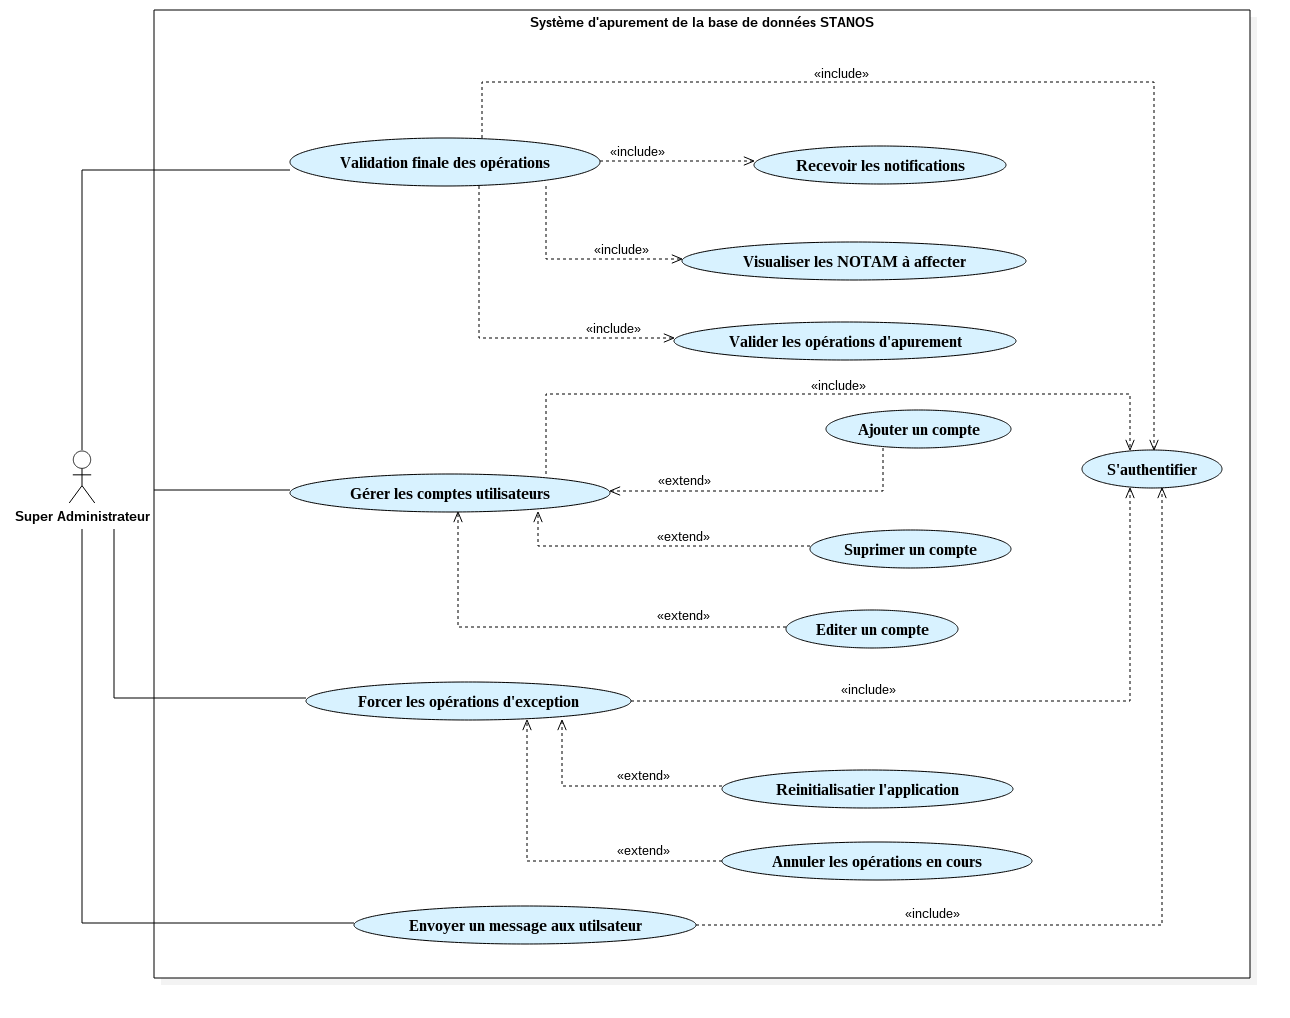
\includegraphics[width=18cm,height=16cm]{besoins/super_administrateur.png}
\end{center}
%légende de l'image
\caption{Diagramme cas d'utilisation pour le super administrateur}
\end{figure}


\subsubsection{Diagramme cas d'utilisation pour l'administrateur}

Le diagramme ci-dessous illustre les cas d’utilisation pour un exploitant de type administrateur. Cet acteur peut effectuer trois différentes actions après avoir s’authentifié. Il valide, alors, d’une manière préliminaire les opérations d’apurement suggéré par l’agent, suggère des modifications sur la liste d’utilisateur et communiquer par messages avec les autres exploitants.\\


\begin{figure}[!h]
\begin{center}
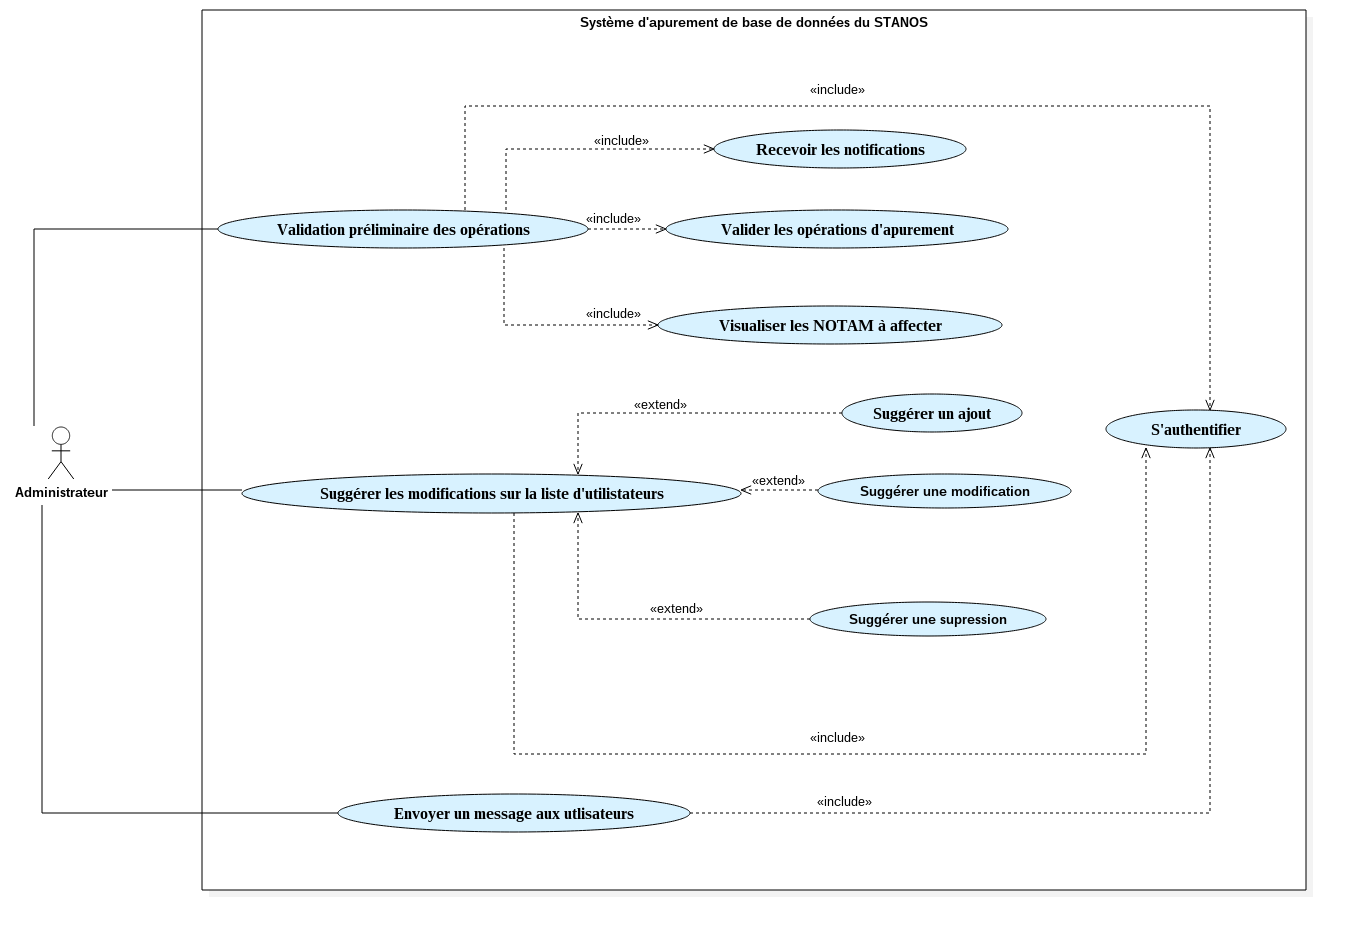
\includegraphics[width=17cm,height=17cm]{besoins/administrateur.png}
\end{center}
%légende de l'image
\caption{Diagramme cas d'utilisation pour l'administrateur}
\end{figure}


\subsubsection{Diagramme cas d'utilisation pour l'agent}

Le diagramme ci-dessous présente les cas d’utilisation pour un agent. Un agent peut effectuer les opérations suivantes après avoir s’authentifié (quoiqu’il soit un agent de site central ou des sites distants) ; lancer des requêtes de mise à jour, valider et tester les lignes sélectionnées et communiquer avec les autres utilisateurs avec messages. Avant de lancer les requêtes d’apurement, un agent site central effectue les opérations suivantes : Création d’un serveur virtuel AIXX, importer la base de AITC vers AIXX et finalement valider les tables NOTAM et PIB. Pour un agent site distant, les opérations à effectuer sont ; sauvegarder une copie de la base existante puis la supprimer, finalement il crée une nouvelle base à partir des lignes validées.

\begin{figure}[!h]
\begin{center}
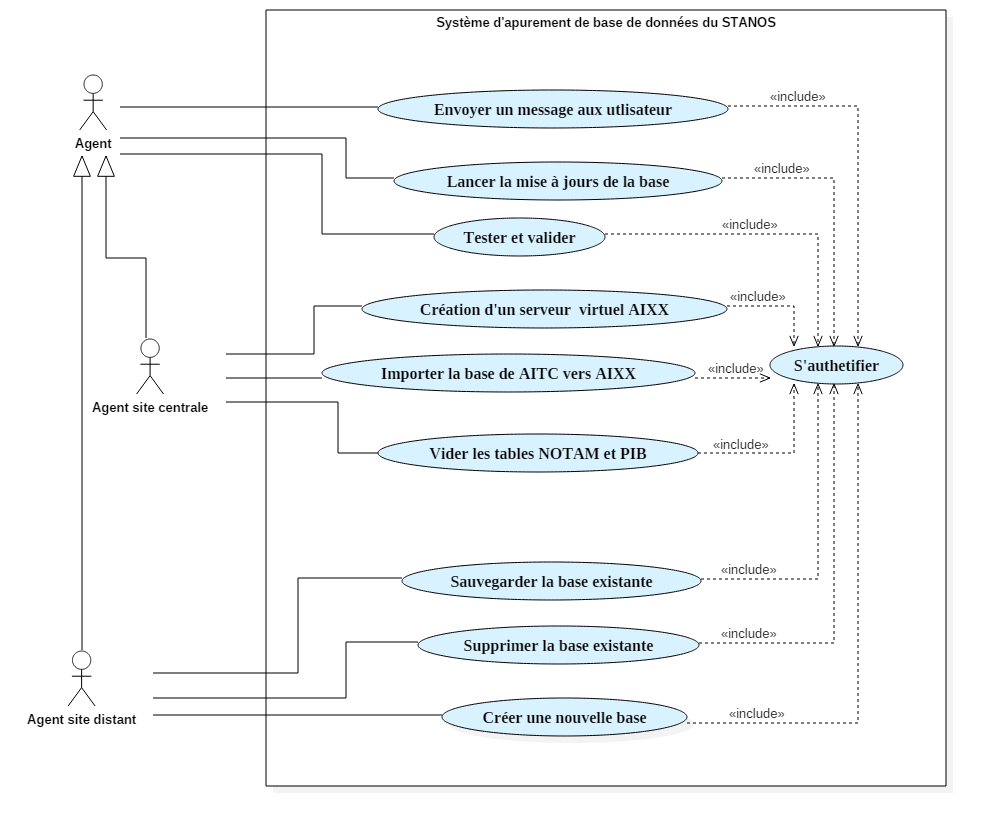
\includegraphics[width=17cm,height=17cm]{besoins/UseCaseDiagram1.png}
\end{center}
%légende de l'image
\caption{Diagramme cas d'utilisation pour l'agent}
\end{figure}
\
\subsection{Diagrammes de séquences système}
Le diagramme de séquence système consiste à décrire l’interaction globale entre le système et l’exploitant. Dans notre système, au premier lieu, l’utilisateur doit fournir séparément un login et un mot de passe pour s’authentifier. Le système vérifie le login et le mot de passe. En cas de correspondance, l’utilisateur est autorisé à accéder aux ressources demandées. Sinon il reste bloqué jusqu’à réussir son authentification.
\begin{figure}[!h]
\begin{center}
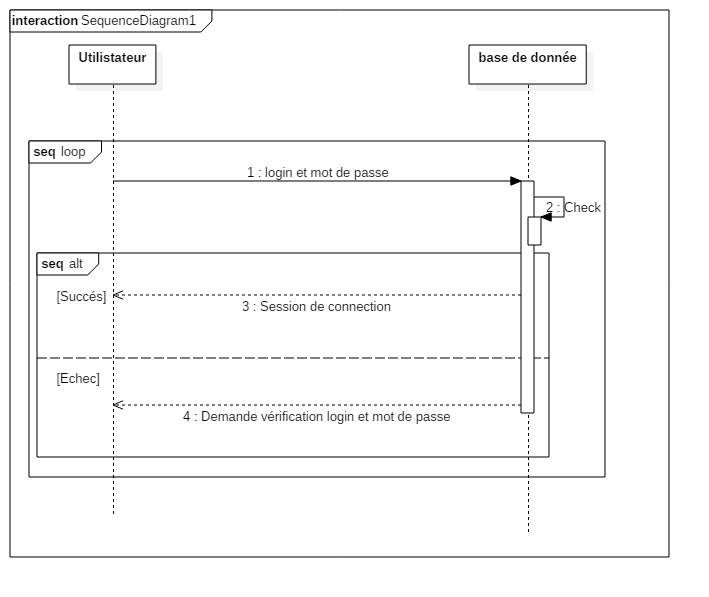
\includegraphics[width=15cm,height=11cm]{Conception/SequenceDiagram2.png}
\end{center}
%légende de l'image
\caption{Diagramme de séquence système}
\end{figure}
\newpage
\subsection*{Conclusion}
Dans ce chapitre nous nous sommes intéressés à l'analyse des besoins fonctionnels et non fonctionnels de notre application. D'autre part, nous avons décelé les cas d'utilisation ainsi que l'acteur principal de l'application et nous avons tracé un diagramme de cas d'utilisation regroupant de manière schématique cette analyse. Enfin, nous avons distingué les différents scénarios qui peuvent avoir lieu, et les dialogues possibles entre le système et le superviseur.









